\documentclass[12pt,a4paper,oneside]{article}
\usepackage{amssymb}
\usepackage{amsthm}
\usepackage[utf8]{inputenc}
\usepackage[danish]{babel}
\usepackage{mathtools}
\usepackage{fancyhdr}
\usepackage[danish]{isodate}
\usepackage{graphicx}
\usepackage{color}

\definecolor{gray}{rgb}{0.5,0.5,0.5}
\usepackage{listings}

\setlength{\parindent}{0pt}

\author{Bertram A. Nicolas}

\newcommand{\Opgn}{5}


\lstset{
  frame=tb,
  language=ML,
  aboveskip=3mm,
  belowskip=3mm,
  showstringspaces=false,
  columns=flexible,
  basicstyle={\small\ttfamily},
  numbers=left,
  numberstyle=\tiny,
  keywordstyle=\color{blue},
  commentstyle=\color{gray},
  stringstyle=\color{red},
  breaklines=true,
  breakatwhitespace=true
  tabsize=4
}

\pagestyle{fancy}
\fancyhf{}
\setlength{\headheight}{2.5em}
\setlength{\headsep}{3em}
\fancyhead[R]{\small \Opgn. hjemmeopgave; 2014 HCI \\
Bertram André Nicolas \& Christian Enevoldsen}
\renewcommand{\headrulewidth}{0pt}

\fancyfoot[L]{\today}
\fancyfoot[C]{\thepage}
\fancyfoot[R]{}

\renewcommand{\thesubsection}{}
\renewcommand{\thesubsubsection}{$\bullet${}}
\begin{document}
\section{Fremgangsmåde}
Tjeklisten mangler at spørge om brugeren synes at løsningen vil få passagererne til ikke at føle ventetiden, og give den offentlige transport et bedre image.
Til sidst mangler vi også at skulle spørge om brugeren selv ville bruge systemet, hvis det blev sat op.
\section{Resultat af indledende PACT-analyse}
\subsection{People}
\begin{itemize}
\item Folk der kører i bus, inklusiv handicappede
\end{itemize}
\subsection{Activities}
\begin{itemize}
\item Det skal være muligt at planlægge en rejse
\item Man skal kunne se køreplaner for bus, tog og metro
\item Køretider for relevante busser skal være tilgængelige
\item Der skal være muligt at se dato og tid i forhold til bussernes køretid
\item Det skal være muligt at kunne følge bussernes kørsel live. (gps)
\item Det skal være muligt at kunne tjekke ud med sit rejsekort
\item Der skal være en guide til billetbestilling på mobil
\item Det skal være muligt at få væsentlige informationer omkring ændringer i køreplaner
\end{itemize}
\subsection{Context}
\begin{itemize}
\item Skærmene er placeret ved busstoppesteder
\item Den skal være brugbar i alle typer vejr
\item Den skal kunne bruges i både i direkte sol og om natten.
\item Der vil være meget trafikstøj
\item Den skal være hurtig, da brugerne kan have travlt
\item Den skal være simpel at bruge, da brugerne ikke har tid til at sætte sig ind i et kompliceret system
\end{itemize}
\subsection{Technology}
\begin{itemize}
\item Det er en touch screen skærm. Der er intet tastatur
\item Skærmen måler 20x30 cm
\item Den har forbindelse til en central, som kan give dugfriske data
\end{itemize}


\section{Tjekliste til interview}
\subsection{Introduktion:}
Bertram og Christian. Fra datalogisk institut, KU. Vi er her i forbindelse med kurset menneske-datamaskine interaktion, hvor vi har til opgave at lave et interview omkring et fiktivt system movia kunne finde på at indføre.
\subsection{Baggrundsoplysninger:}
\subsection{Navn:}
\subsection{Stilling:}
\subsection{IT-erfaring:}
\begin{itemize}
\item Bruger du PC til daglig?
\item Ejer du en smartphone eller tablet?
\begin{itemize}
\item Ved du hvordan touch fungerer?
\end{itemize}
\item Hvordan løser du et problem med computeren?
\item Har du lavet et program selv eller har du programmeret før?
\item Hvor ofte kører du med bus?
\item Hvordan finder du information omkring bustider og forsinkelser?
\begin{itemize}
\item Hvordan sysnes du det fungerer?
\end{itemize}
\end{itemize}
\subsection{Det nye system:}
\begin{itemize}
\item Hvordan kan oplevelsen af ventetid forbedres ved busstoppestederne?
\end{itemize}
\subsection{Præsentation af det nye system:}
Movia har tænkt sig at lave et nyt system, som skal få passagererne til ikke at føle ventetiden når de venter på bussen.
\begin{itemize}
\item Det er en touch screen. Der er intet Tastatur
\item Skærmen måler 20x30 cm (a4)
\item Den har forbindelse til en central, som kan give dugfriske data.
\end{itemize}
\subsection{Vi har tænkt at den skal kunne flg.:}
\begin{itemize}
\item Det skal være muligt at planlægge en rejse
\item Man sal kunne se køreplaner for bus, tog og metro.
\item Køretider for relevante busser skal være tilgængelige
\item Det skal være muligt at kunne følge bussernes kørsel live. (gps)
\item Det skal være muligt at kunne tjekke ud med sit rejsekort
\item Det skal være muligt at får væsentlige informationer omkring ænringer i køreplanerne.
\end{itemize}
\subsection{Afsluttende spørgsmål:}
\begin{itemize}
\item Hvad synes du om denne ide?
\item Hvordan kunne dette forbedres?
\item Hvordan tror du at denne løsning vil påvirke passagererne der venter på bussen?
\item Hvordan tror du at denne løsning vil påvirke den offentlige transports image?
\item Hvilke dele af systemet ville du selv bruge?
\end{itemize}
\section{Interviewresultater}

\begin{enumerate}
\item{Det skal være simpelt og hurtigt.}
\item{Oversigt med opdateringer skal være tilgængelige på alle skærme (selvom en er igang med at tjekke ud for eksempel)}
\item{Planlægning af ruter behøves ikke, da det er for kompleks, og der skal være plads til at mange kan bruge systemet på en gang.}
\item{Zoneoversigt med mulighed for at zoome, så folk med dårligt syn også kan se hvad der står.}
\item{Alle skal kunne bruge det.}
\item{GPS og tjek ud delen er det de fleste vil sætte pris på.}
\end{enumerate}

\textbf{Forståelse af brugernes behov.}

Ud fra vores interviews fremgår det klart og tydeligt, at check ud og GPS oversigten er det mest væsentlige for brugerne.
Det skal være mere oversigtsagtigt end det skal være interaktivt, da der er mange brugere som bruger det på samme tid.
På baggrund af vores interviews sætter folk mest pris på at opdateringer, live gps og check ud.\newline


Sådan lyder det fra interviewdeltagerne: 
Undgå touchscreen, se et kort hvor bussen er.
News feed scrollers med forsinkelser.
eventuelt gøre så man altid kan se de vigtigste informationer selvom der er en anden bruger der aktivt er i gang med systemet.\newline


Forsinkelser bliver mere positive, når man kan følge med i hvad der er sket og hvor langt busserne er.
Folk kan lettere planlægge nye rejser
folk vil bruge flere alternative ruter
Det anses ikke som et problem at vente på busser når der ikke er forsinkelser.\newline

For folk som hader at vente på bussen, vil systemet ikke gøre en forskel, mener Kasper Hansen.
De nuværende nedtællere er ikke præcise nok. Når der står 3 minutter tilbage og der så er gået 7 minutter, bliver folk frustreret fordi der underforstået er blevet lovet noget som ikke blev holdt. Derfor er det vigtigt at meddele folk om at det er en anslået tid, eller endnu bedre: vær præcis med tiderne. 
Det kunne være en ide at undgå nedtællinger, men derimod give info omkring forsinkelser i stedet. Folk kan jo som sagt følge med hvor bussen er.

\section{Kerneopgaver}

\begin{enumerate}
\item {(forfalden på baggrund af interviews) Det skal være muligt at planlægge en rejse}
\item {Man skal kunne se køreplaner for bus, tog og metro}
\item {Køretider for relevante busser skal være tilgængelige}
\item {Det skal være muligt at kunne følge bussernes kørsel live (gps)}
\item {Det skal være muligt at kunne tjekke ud med sit rejsekort}
\item {Det skal være muligt at få væsentlige informationer omkring ændringer i
køreplaner}\newline

\textbf{Tilføjet efter interview}

\item {Man skal kunne se en oversigt over zoner. Ligesom på prototypen}
\end{enumerate}


\section{Målgrupper og målgruppebeskrivelse}
\section{Personas}
\section{Scenarier}
\section{Prototype}
Billederne er også vedlagt som rå filer i mappen img.

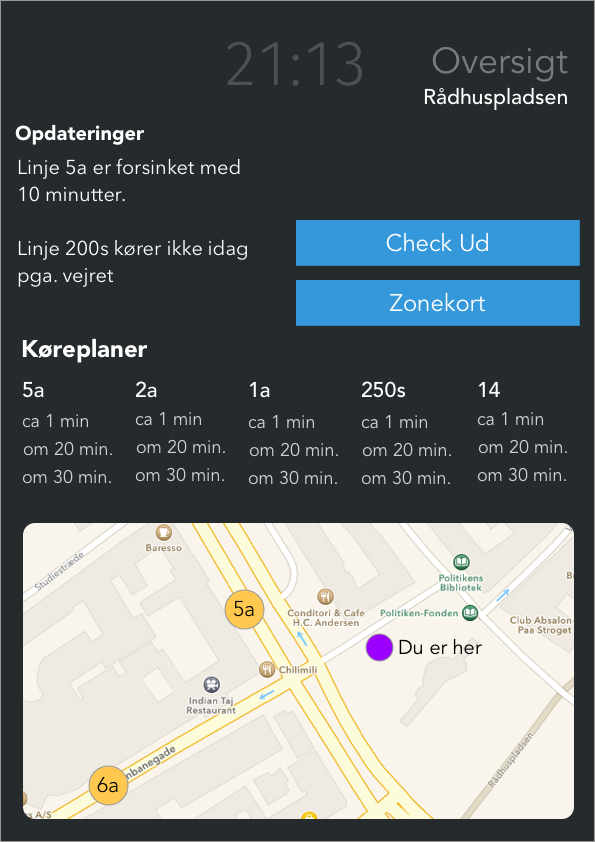
\includegraphics[scale=0.5]{img/Oversigt.png}\newpage
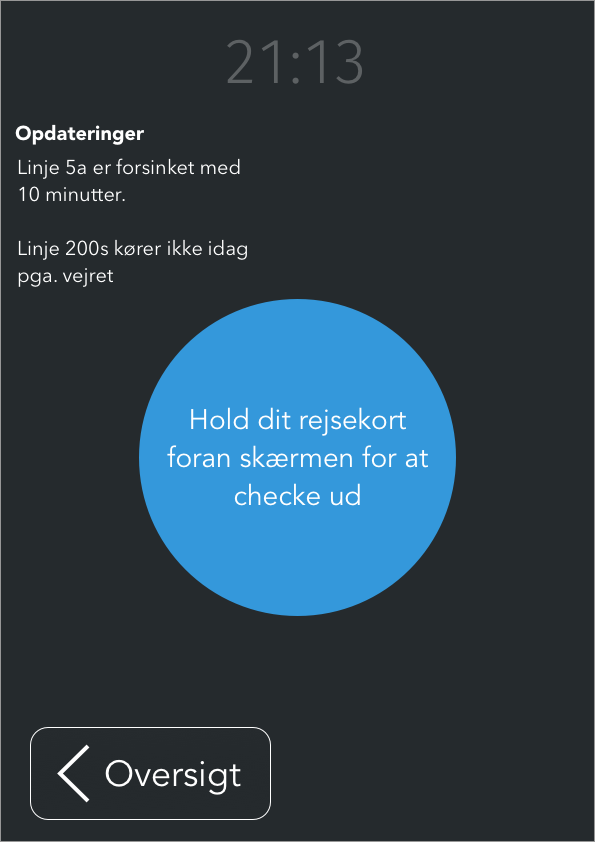
\includegraphics[scale=0.5]{img/CheckUd.png}\newpage
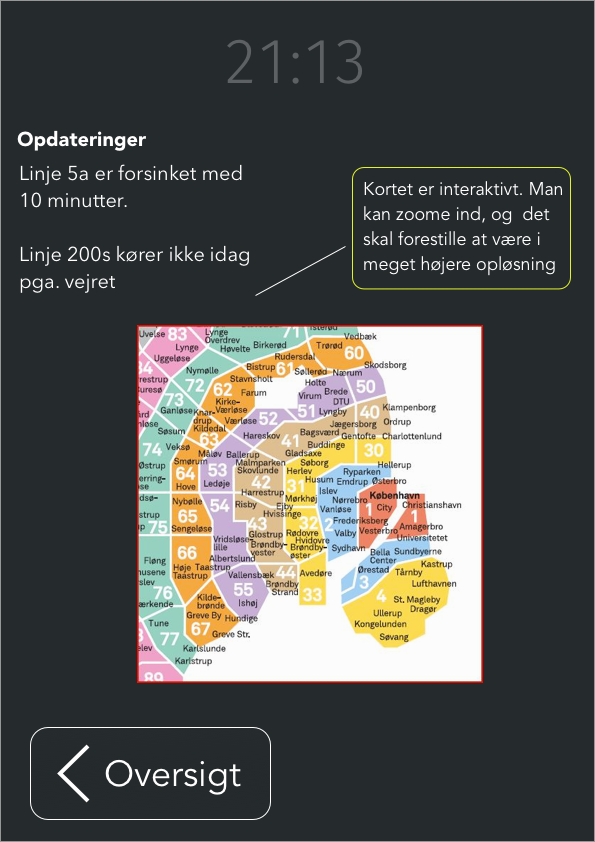
\includegraphics[scale=0.5]{img/Zonekort.png}\newpage


\section{Erfaringer}
\section{Appendiks: Kommentarer}
\end{document}